\section{Completed results}
\subsection{Primary clean comparison}
All twelve scientific trajectories complete their declared 600 updates, and all sixty fold-specific evaluation groups are retained. Thirty pooled SDK scopes merge unique-token boxes; no fold AP is averaged. Tables~\ref{tab:new_main_clean}--\ref{tab:new_primary_per_log} report every primary seed, arm, and capture log. The custom outer support is 1,347 pedestrian and 1,590 joint-VRU annotation observations in 162 frames, with 137 joint-target frames. The same observations recur across seeds.

% Generated from analysis/results.json SHA256 da5dbfb0c658a72ddddfcfc12c54ac1523bfc23094f806cef8627830b8c851da
% Generated from mechanism/RESULTS.json SHA256 3c491671a72237b819dfa725a969a978ade9430f347126e4bc921b0f9215186f
% Generated from mechanism/INFERENCE_GATE_STATISTICS.csv SHA256 445a4a298458eaf9d99f4981eca4be1b3ae5389261a8e0870aab6ee421249b43
% Generated from make_paper_tables.py SHA256 c0379ecdaac1296f16b841f096afbfa02ce6dc80253739e3b3da0d99554dfba0
\begin{table*}[t]
\centering
\footnotesize
\setlength{\tabcolsep}{3.3pt}
\caption{Fixed clean outer panel on historically exposed nuScenes mini: all 162 frames/four logs, separately for every seed. SDK mAP/NDS/pedAP are percentages computed from pooled boxes, never fold-averaged AP. Pedestrian/joint hits and joint AnyMiss retain their observation/target-frame denominators. Saved and all-range unmatched pedestrian outputs use score $\geq0.1$; they are output burden, not official false positives or precision. Neutral has no new adaptation and is not an equal-update control. The three seeds reuse the same logs; their counts must not be summed as independent data. NA denotes unavailable or unsupported values.}
\label{tab:new_main_clean}
\begin{tabular}{clrrrrrrrr}
\toprule
Seed & Arm & mAP & NDS & PedAP & Ped. hits & Joint hits & AnyMiss & Saved ped. & Unmatched ped. \\
\midrule
0 & Neutral & 1.671 & 8.606 & 2.950 & 442/1347 & 478/1590 & 128/137 & 5836 & 5374 \\
0 & Constant & 1.621 & 8.675 & 2.419 & 410/1347 & 448/1590 & 131/137 & 4898 & 4471 \\
0 & Dynamic & 1.617 & 8.605 & 2.447 & 408/1347 & 446/1590 & 131/137 & 4920 & 4494 \\
1 & Neutral & 1.698 & 8.042 & 3.974 & 513/1347 & 542/1590 & 122/137 & 7512 & 6975 \\
1 & Constant & 1.713 & 7.826 & 3.693 & 486/1347 & 520/1590 & 124/137 & 6537 & 6030 \\
1 & Dynamic & 1.710 & 7.843 & 3.681 & 488/1347 & 523/1590 & 125/137 & 6529 & 6020 \\
2 & Neutral & 1.935 & 7.811 & 3.978 & 462/1347 & 488/1590 & 127/137 & 6305 & 5822 \\
2 & Constant & 1.880 & 7.002 & 3.662 & 424/1347 & 453/1590 & 130/137 & 5527 & 5085 \\
2 & Dynamic & 1.879 & 6.998 & 3.721 & 433/1347 & 462/1590 & 130/137 & 5553 & 5102 \\
\bottomrule
\end{tabular}
\end{table*}

% Generated from analysis/results.json SHA256 da5dbfb0c658a72ddddfcfc12c54ac1523bfc23094f806cef8627830b8c851da
% Generated from mechanism/RESULTS.json SHA256 3c491671a72237b819dfa725a969a978ade9430f347126e4bc921b0f9215186f
% Generated from mechanism/INFERENCE_GATE_STATISTICS.csv SHA256 445a4a298458eaf9d99f4981eca4be1b3ae5389261a8e0870aab6ee421249b43
% Generated from make_paper_tables.py SHA256 c0379ecdaac1296f16b841f096afbfa02ce6dc80253739e3b3da0d99554dfba0
\begin{table*}[t]
\centering
\footnotesize
\setlength{\tabcolsep}{4.0pt}
\caption{Primary clean dynamic-minus-constant contrast, with the same historically exposed panel in each seed. Recall differences are percentage points (pp). Recovery/loss/persistent-miss counts are annotation observations, not distinct people. Equal-count swaps count pedestrian-containing frames with both recovered and newly lost matches despite unchanged hit totals. Joint clear/new counts are exact all-clear recoveries/newly failed frames. No seed or endpoint is selected by sign.}
\label{tab:new_primary_decomposition}
\begin{tabular}{crrrrrrrr}
\toprule
Seed & $\Delta R_{\rm ped}$ & $\Delta R_{\rm equal\ log}$ & Recovered & Newly lost & Persist. miss & Equal-count swaps & Joint clear & Joint new \\
\midrule
0 & -0.148 & -0.157 & 5 & 7 & 932 & 2 & 0 & 0 \\
1 & +0.148 & -0.227 & 5 & 3 & 856 & 1 & 0 & 1 \\
2 & +0.668 & +0.796 & 9 & 0 & 914 & 0 & 0 & 0 \\
\bottomrule
\end{tabular}
\end{table*}

% Generated from analysis/results.json SHA256 da5dbfb0c658a72ddddfcfc12c54ac1523bfc23094f806cef8627830b8c851da
% Generated from mechanism/RESULTS.json SHA256 3c491671a72237b819dfa725a969a978ade9430f347126e4bc921b0f9215186f
% Generated from mechanism/INFERENCE_GATE_STATISTICS.csv SHA256 445a4a298458eaf9d99f4981eca4be1b3ae5389261a8e0870aab6ee421249b43
% Generated from make_paper_tables.py SHA256 c0379ecdaac1296f16b841f096afbfa02ce6dc80253739e3b3da0d99554dfba0
\begin{table*}[t]
\centering
\footnotesize
\setlength{\tabcolsep}{5.0pt}
\caption{Every primary clean seed/log contrast on the fixed panel. C and D denote constant and dynamic gates. Pedestrian hit and joint AnyMiss fractions retain their respective denominators; recall differences are pp. Log IDs are unique eight-character prefixes of the full tokens in the companion records. The same four logs recur across the three model seeds, with repeated observations within logs; rows are descriptive, not independent replications.}
\label{tab:new_primary_per_log}
\begin{tabular}{clrrrrr}
\toprule
Seed & Log prefix & Ped. hits C & Ped. hits D & $\Delta R_{\rm ped}$ & Joint AnyMiss C & Joint AnyMiss D \\
\midrule
0 & \texttt{5bd40b61} & 121/383 & 120/383 & -0.261 & 26/26 & 26/26 \\
0 & \texttt{6f7fe59a} & 14/67 & 14/67 & 0.000 & 27/31 & 27/31 \\
0 & \texttt{7e25a2c8} & 114/623 & 114/623 & 0.000 & 39/39 & 39/39 \\
0 & \texttt{881dd2f8} & 161/274 & 160/274 & -0.365 & 39/41 & 39/41 \\
1 & \texttt{5bd40b61} & 153/383 & 152/383 & -0.261 & 26/26 & 26/26 \\
1 & \texttt{6f7fe59a} & 33/67 & 32/67 & -1.493 & 20/31 & 21/31 \\
1 & \texttt{7e25a2c8} & 116/623 & 119/623 & +0.482 & 39/39 & 39/39 \\
1 & \texttt{881dd2f8} & 184/274 & 185/274 & +0.365 & 39/41 & 39/41 \\
2 & \texttt{5bd40b61} & 118/383 & 118/383 & 0.000 & 26/26 & 26/26 \\
2 & \texttt{6f7fe59a} & 23/67 & 24/67 & +1.493 & 26/31 & 26/31 \\
2 & \texttt{7e25a2c8} & 95/623 & 101/623 & +0.963 & 39/39 & 39/39 \\
2 & \texttt{881dd2f8} & 188/274 & 190/274 & +0.730 & 39/41 & 39/41 \\
\bottomrule
\end{tabular}
\end{table*}


Dynamic-minus-constant pedestrian recall changes are $-0.148$, $+0.148$, and $+0.668$ percentage points (pp), corresponding to $-2,+2,+9$ hits. None reaches the required $+1$ pp. Joint AnyMiss remains $131/137$ for seed~0 and $130/137$ for seed~2, but rises from $124/137$ to $125/137$ for seed~1. Saved pedestrian-output ratios are 1.00449, 0.99878, and 1.00470, below the burden ceiling. Passing that ceiling does not rescue failure of the other conjunctive conditions.

Equal-log pedestrian changes are $-0.157,-0.227,+0.796$ pp. Seed~1 therefore reverses sign between pooled and equal-log summaries. Table~\ref{tab:new_primary_per_log} makes the log denominators and heterogeneous changes visible; neither a favorable pooled seed nor an individual log replaces the prespecified panel. There are four logs rather than four independent experimental datasets.

The absolute SDK metrics remain low: primary mAP spans approximately 1.62--1.94\% across all three arms. Dynamic-minus-constant changes are small and mixed across mAP, NDS, and pedestrian AP. These SDK endpoints use their own filtering and class support, so their numerical values are not interchangeable with the critical custom recall. Full per-class filtered support, per-fold metrics, and 108 per-log SDK evaluations are retained in the companion. Unsupported classes and empty per-log support remain explicit; no favorable supported subset is promoted as an alternative headline.

\subsection{Recovery, loss, and persistent failures}
The pedestrian recovered/newly-lost pairs are $5/7$, $5/3$, and $9/0$. Joint-VRU pairs are $6/8$, $6/3$, and $9/0$. There are no joint all-clear recoveries in any primary seed, with one new joint failure in seed~1. Equal-count pedestrian identity exchanges occur in two, one, and zero frames, respectively. Thus identical hit counts and unchanged AnyMiss totals do not establish identical matched targets.

\begin{figure*}[t]
\centering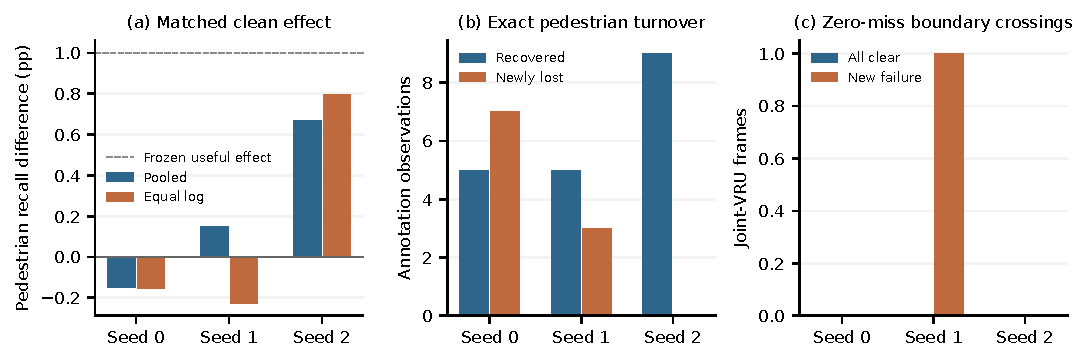
\includegraphics[width=\textwidth]{images/primary_identity_effects.pdf}
\caption{All three primary clean seeds: pooled and equal-log pedestrian effects, exact recovered/newly-lost annotation observations, and joint failed-frame changes. The same 162-frame historical panel is reused. Counts refer to matcher assignments, not distinct people or independently sampled frames.}\label{fig:primary}
\end{figure*}

The number of frames with improved pedestrian hit counts is three, four, and eight. Every such frame still misses at least one pedestrian. All five, five, and nine recovered pedestrian observations, respectively, occur on frames that remain joint failures, including recoveries in equal-count exchange frames. Seed~2 is especially instructive: nine recovered observations and no newly lost pedestrians improve recall, yet all nine occur on still-failed frames and AnyMiss remains unchanged. This is direct endpoint accounting, not evidence about the physical severity of those misses.

\begin{figure*}[t]
\centering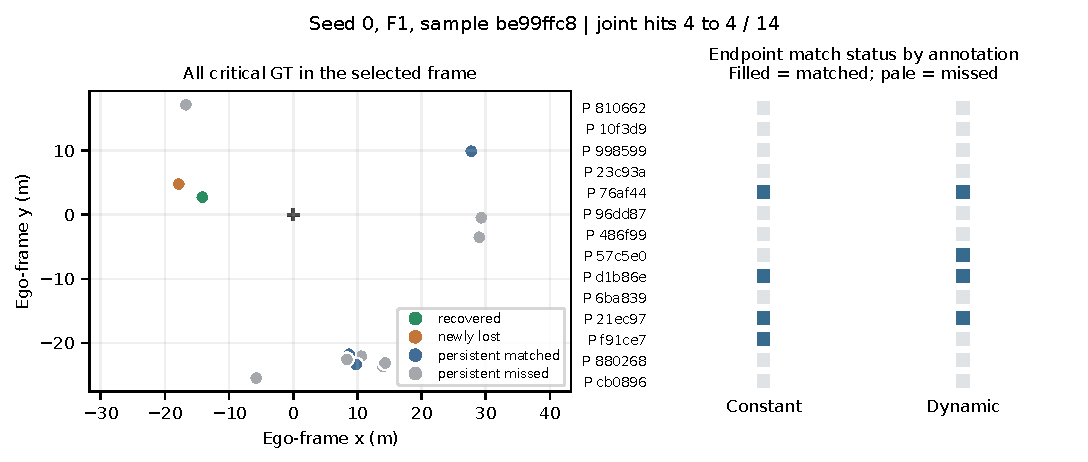
\includegraphics[width=0.96\textwidth]{images/identity_case.pdf}
\caption{Deterministically selected identity illustration: seed~0, clean F1 frame \texttt{be99ffc878b24aca8956bbb4e0f97d0c}. Among 14 critical pedestrian annotations, both arms match four and miss ten; one annotation is recovered and another newly lost. The left panel locates annotations in ego coordinates; the right panel shows the 14 matched-status assignments. P denotes pedestrian and suffixes abbreviate annotation IDs. Selection uses the first lexicographic qualifying frame with at most 20 targets, prioritizing equal-count identity exchange; it selects an illustration, not a model or outcome estimate. Colors encode the declared matcher, without image-based adjudication or cross-run prediction tracking.}\label{fig:case}
\end{figure*}

\subsection{Secondary views and the neutral parent}
% Generated from analysis/results.json SHA256 da5dbfb0c658a72ddddfcfc12c54ac1523bfc23094f806cef8627830b8c851da
% Generated from mechanism/RESULTS.json SHA256 3c491671a72237b819dfa725a969a978ade9430f347126e4bc921b0f9215186f
% Generated from mechanism/INFERENCE_GATE_STATISTICS.csv SHA256 445a4a298458eaf9d99f4981eca4be1b3ae5389261a8e0870aab6ee421249b43
% Generated from make_paper_tables.py SHA256 c0379ecdaac1296f16b841f096afbfa02ce6dc80253739e3b3da0d99554dfba0
\begin{table*}[t]
\centering
\footnotesize
\setlength{\tabcolsep}{3.5pt}
\caption{All fixed secondary dynamic-minus-constant views; SDK differences and pedestrian recall changes are pp. L50: outer LiDAR retention 0.5; Dec0: clean outer inference with decoder LiDAR input half zeroed; Dev: the original development roles, with different support shown explicitly. The support column is frames/pedestrian observations/joint-VRU observations. AnyMiss shows C$\to$D divided by target-containing frames, and burden is saved-pedestrian D/C. Dec0 is an inference intervention, not a retrained path-free comparison; Dev is descriptive and does not select checkpoints. These historically exposed, repeated seed populations are not independent data. NA denotes undefined, unavailable or unsupported values.}
\label{tab:new_secondary}
\begin{tabular}{ccrrrrrrr}
\toprule
View & Seed & Frames/Ped/Joint & $\Delta$ mAP & $\Delta$ NDS & $\Delta$ PedAP & $\Delta R_{\rm ped}$ & AnyMiss C$\to$D / N & Burden D/C \\
\midrule
L50 & 0 & 162/1347/1590 & +0.005 & -0.013 & +0.014 & -0.371 & $131\!\to\!131\;/\;137$ & 1.005 \\
L50 & 1 & 162/1347/1590 & +0.001 & +0.172 & -0.005 & +0.223 & $125\!\to\!124\;/\;137$ & 0.998 \\
L50 & 2 & 162/1347/1590 & -0.002 & +0.002 & +0.068 & +0.371 & $128\!\to\!127\;/\;137$ & 1.008 \\
Dec0 & 0 & 162/1347/1590 & -0.002 & +0.007 & +0.038 & -0.148 & $134\!\to\!134\;/\;137$ & 0.998 \\
Dec0 & 1 & 162/1347/1590 & -0.002 & +0.168 & +0.013 & +0.223 & $127\!\to\!127\;/\;137$ & 0.996 \\
Dec0 & 2 & 162/1347/1590 & 0.000 & +0.054 & +0.039 & +0.297 & $128\!\to\!128\;/\;137$ & 1.002 \\
Dev & 0 & 82/315/336 & +0.020 & +0.018 & -0.054 & -1.270 & $61\!\to\!61\;/\;65$ & 0.999 \\
Dev & 1 & 82/315/336 & +0.014 & -0.008 & +0.131 & +0.952 & $64\!\to\!64\;/\;65$ & 1.002 \\
Dev & 2 & 82/315/336 & +0.077 & +0.035 & +0.231 & 0.000 & $57\!\to\!57\;/\;65$ & 1.004 \\
\bottomrule
\end{tabular}
\end{table*}

Table~\ref{tab:new_secondary} preserves every fixed secondary row. Under 50\% LiDAR retention, the three pedestrian effects are $-0.371,+0.223,+0.371$ pp, with joint failure changes $0,-1,-1$. Decoder-half masking gives $-0.148,+0.223,+0.297$ pp and no dynamic--constant failure-count changes. Development effects are $-1.270,+0.952,0.000$ pp; none changes joint failure counts. These views were completed without adapting the schedule, gate, or checkpoint to their outcomes.

\begin{figure*}[t]
\centering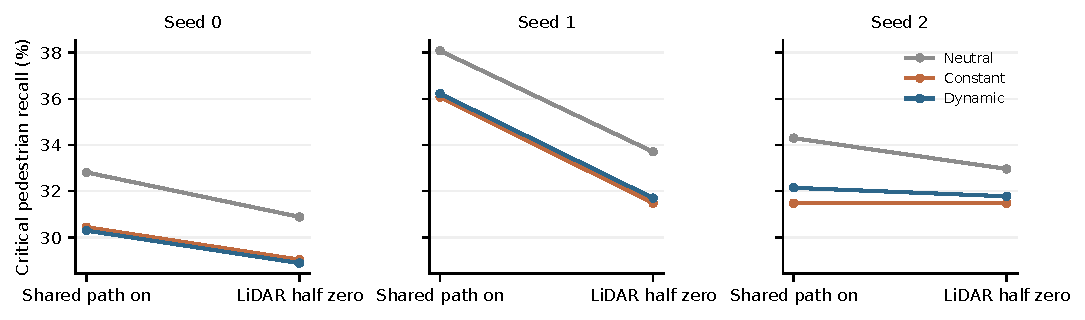
\includegraphics[width=\textwidth]{images/decoder_intervention.pdf}
\caption{Same-checkpoint decoder LiDAR input intervention for all evaluated clean arms and seeds. Encoder LiDAR remains enabled. Changes measure sensitivity to this masking operation on a detector trained with the route, not the effect of retraining without it or a decomposition of predictive contribution.}\label{fig:decoder}
\end{figure*}

Compared with its unadapted U8000 parent, each adapted arm has fewer primary pedestrian and joint hits and more joint failed frames (Table~\ref{tab:new_main_clean}). Saved outputs also decrease. This establishes no practical improvement over the inherited detector under the chosen short adaptation schedule. The neutral parent has zero new updates rather than 600; the comparison cannot isolate the gate, encoder adaptation, optimization schedule, or their interaction as the cause. Reduced output burden is not an official precision improvement.

\section{Observed gate and path behavior}
% Generated from analysis/results.json SHA256 da5dbfb0c658a72ddddfcfc12c54ac1523bfc23094f806cef8627830b8c851da
% Generated from mechanism/RESULTS.json SHA256 3c491671a72237b819dfa725a969a978ade9430f347126e4bc921b0f9215186f
% Generated from mechanism/INFERENCE_GATE_STATISTICS.csv SHA256 445a4a298458eaf9d99f4981eca4be1b3ae5389261a8e0870aab6ee421249b43
% Generated from make_paper_tables.py SHA256 c0379ecdaac1296f16b841f096afbfa02ce6dc80253739e3b3da0d99554dfba0
\begin{table*}[t]
\centering
\footnotesize
\setlength{\tabcolsep}{4.0pt}
\caption{Realized fixed-checkpoint gate behavior on clean outer frames, for every fold/seed. The dynamic SD column is the largest across-frame coefficient standard deviation among the four layers (pp), not variation across layers within one frame. Maximum baseline deviation is the largest absolute dynamic change (pp). Constant SD is defined identically. Boundary occupancy is the largest layer fraction (\%) at $\geq99\%$ of that layer's allowed amplitude. The absolute coefficient bound is at most 10 pp, reduced near probability boundaries. These are descriptions of historically exposed frames, not efficacy estimates or independent samples.}
\label{tab:new_mechanisms}
\begin{tabular}{ccrrrrr}
\toprule
Fold & Seed & Frames & Dynamic max SD (pp) & Max deviation (pp) & Constant max SD (pp) & Boundary occupancy (\%) \\
\midrule
F1 & 0 & 80 & 0.34008 & 2.015 & 0.00000 & 0.000 \\
F1 & 1 & 80 & 0.21272 & 1.356 & 0.00000 & 0.000 \\
F1 & 2 & 80 & 0.17068 & 1.734 & 0.00000 & 0.000 \\
F2 & 0 & 82 & 0.31229 & 1.844 & 0.00000 & 0.000 \\
F2 & 1 & 82 & 0.20672 & 1.130 & 0.00000 & 0.000 \\
F2 & 2 & 82 & 0.24261 & 2.633 & 0.00000 & 0.000 \\
\bottomrule
\end{tabular}
\end{table*}

Training telemetry agrees with neutral initialization: all twelve runs have positive first-update output-head gradient norms, while all 36 recorded descriptor/projection/hidden module groups have zero first-update gradients. Earlier module gradients subsequently become positive in all twelve runs. These observations verify that the intended learning paths activate; they do not establish useful conditioning.

At the fixed final checkpoints, the largest across-frame coefficient SD among four layers ranges from 0.17068 to 0.34008 pp over the six dynamic fold/seed models. The largest absolute departure from an inherited coefficient ranges from 1.130 to 2.633 pp. Constant descriptors yield zero across-frame coefficient SD. No recorded clean outer coefficient reaches 99\% of its allowed amplitude. The realized dynamic gate is therefore frame-dependent and remains well inside its bound on these frames; bound saturation does not describe the observed weak result. No matched unbounded experiment identifies what an alternative amplitude would do.

The same checkpoint produces identical coefficients before and after decoder-input masking because the intervention occurs downstream of gate computation. The recorded pre-mask encoder and decoder-LiDAR input norms establish that both inputs are present. LayerNorm scaling and norms are not calibrated contribution fractions: their magnitude cannot establish LiDAR dominance, gate redundancy, or causal responsibility. Masking changes detector outcomes, but a retrained route-free model could behave differently. The isolated all-camera-masks-empty forward check returns exactly $2q$ in evaluation; this narrowly verifies the audited branch and says nothing about its frequency or metric impact in the real panel.
